% Setup -------------------------------

\documentclass[a4paper]{report}
\usepackage[a4paper, total={6in, 10in}]{geometry}
\setcounter{secnumdepth}{3}
\setcounter{tocdepth}{3}

\usepackage{indentfirst}

\usepackage[hyphens]{url}
\usepackage{hyperref}

\usepackage{titlepic}

\usepackage{graphicx}
\usepackage{float}
\usepackage{minted}
\usepackage{xcolor}

\usepackage{tikz}
\usetikzlibrary{trees}
\tikzstyle{every node}=[draw=black,thick,anchor=west]
\tikzstyle{selected}=[draw=orange,fill=orange!30]
\tikzstyle{root}=[draw=red,fill=red!30]

\definecolor{friendlybg}{HTML}{f0f0f0}
\setminted[yaml]{
	style=manni,
	bgcolor=friendlybg,
	linenos,
	frame=lines,
	framerule=0.6pt,
	framesep=5pt,
	rulecolor=orange,
	fontsize=\footnotesize
}

% Encoding
%--------------------------------------
\usepackage[T1]{fontenc}
\usepackage[utf8]{inputenc}
%--------------------------------------

% Portuguese-specific commands
%--------------------------------------
\usepackage[portuguese]{babel}
%--------------------------------------

% Hyphenation rules
%--------------------------------------
\usepackage{hyphenat}
%--------------------------------------

% Capa do relatório

\title{
	Aprendizagem Automática 2
	\\ \Large{\textbf{Trabalho Prático}}
	\\ -
	\\ Mestrado em Engenharia Informática
	\\ Universidade do Minho
}
\author{
	\begin{tabular}{ll}
		\textbf{Grupo nº 11}
		\\
		\hline
		PG41080 & João Ribeiro Imperadeiro
        \\
		PG41081 & José Alberto Martins Boticas
		\\
        PG41091 & Nelson José Dias Teixeira
        \\
        PG41851 & Rui Miguel da Costa Meira
	\end{tabular}
	\vspace{1cm}
}

\date{\today}

\titlepic{
	\vspace{2cm}
	
\includegraphics[scale=0.065]{Images/EEUM_logo.png}
}

\begin{document}

\begin{titlepage}
    \maketitle
\end{titlepage}

% Índice

\tableofcontents
\listoffigures

% Introdução

\chapter{Introdução} \label{ch:Introduction}
\large {
	No âmbito da unidade curricular (UC) \textsl{Aprendizagem Automática II} (AA2), foi requerida a realização de um trabalho prático para avaliação.
	Tal como foi proposto a 23 de abril, o grupo escolheu a opção relativa ao desenvolvimento de algoritmos/\textit{software} no âmbito de aprendizagem máquina.
	Mais especificamente, optou-se pelo desenvolvimento de uma \textit{framework} de \textsl{AutoML}, com o objetivo de obter o melhor modelo para problemas de \textit{supervised learning} e \textit{unsupervised learning}, 
	de forma automática e com a menor intervenção possível por parte do programador. À \textit{framework} idealizada foi atribuído o nome \textsl{UnicornML}.
	
	Atualmente existem já algumas \textit{frameworks} que abordam este tema de forma mais profunda e complexa.
	Destas soluções destacam-se a \textit{Lex}, desenvolvida pela \textit{Amazon} e que disponibiliza funcionalidades de \textit{deep learning} relacionadas com texto e voz, o \textit{AutoKeras}, um sistema de \textsl{AutoML} baseado em \texttt{keras} e, ainda, a \textit{Google AutoML}, que vai ao encontro com o que o grupo deste trabalho pretende realizar.
	Esta última \textit{framework} permite desenvolver modelos para utilizadores que não possuem qualquer conhecimento de \textit{machine learning}. Consequentemente, esta acaba por ser transparente para o cliente na obtenção do resultado obtido.

	Por sugestão do docente da UC, foram postos de parte os problemas de \textit{unsupervised learning}, pela sua complexidade e menor atenção dada durante as aulas.
	Assim, sobram apenas os problemas de \textit{supervised learning} que podem ser divididos em duas categorias: classificação e regressão. Mais à frente serão abordadas as duas categorias em pormenor.
	Para proceder à avaliação dos modelos disponibilizados pela \textit{framework}, adotaram-se algumas métricas para cada um dos tipos de problemas mencionados acima.
	De salientar que o grupo teve o cuidado de avaliar situações relacionadas com o \textit{underfitting} e \textit{overfitting} dos modelos gerados. Para tal foram utilizadas, na generalidade, metodologias intrínsecas à otimização de hiperparâmetros.

	Relativamente à estrutura deste documento, será, de seguida, exibida a planificação deste projeto, definindo alguns dos objetivos a serem alcançados.
	Posteriormente, parte-se para a implementação da \textit{framework} proposta, evidenciando-se questões relacionadas com o pré-processamento de dados, os problemas e algoritmos suportados pela aplicação e também as métricas utilizadas no momento da avaliação dos modelos.
	Por fim, é demonstrada uma análise sobre os vários testes realizados sobre a \textit{framework}, sumariando os objetivos atingidos neste projeto.
}

\chapter{Planificação} \label{ch:Planning}
\large {
	Uma vez feita a escolha acerca do tema que este grupo de trabalho se propôs a efetuar, segue-se a planificação do que vai ser realizado.
	\begin{itemize}
		\item Criação do \textit{package} \textsl{UnicornML} com diversas classes;
		\item Implementação de testes unitários para validar as funcionalidades;
		\item Utilização das bibliotecas \textit{scikit-learn}, \textit{tensorflow} e \textit{kerastuner};
		\item Código \textit{open source} disponível para todos os utilizadores de \texttt{Python} no \textit{PyPI};
		\item Desenvolver uma \textit{framework} que seja capaz de encontrar um modelo com uma exatidão alta;
		\item Implementar uma aplicação simples de utilizar, sendo apenas necessário fornecer os dados;
		\item Garantir a busca do modelo ótimo para um determinado conjunto de dados de forma rápida, eficiente e robusta;
		\item Servir esta \textit{framework} como uma excelente base para um projeto de maiores dimensões.
	\end{itemize}
}

\chapter{Implementação} \label{ch:Implementation}
\large {
	\section{Estrutura} \label{sec:Structure}
    A \textsl{UnicornML} apresenta um estrutura simples e clara, tal como se pode observar no seguinte diagrama.
    
    \begin{figure}[H]
        \centering
        \begin{tikzpicture}[
            grow via three points={one child at (0.5,-0.7) and
            two children at (0.5,-0.7) and (0.5,-1.4)},
            edge from parent path={(\tikzparentnode.south) |- (\tikzchildnode.west)}
        ]
            \node [root] {Code}
                child { node [selected] {data}
                    child { node {...} }
				}
				child [missing] {}
				child { node [selected] {tests}
					child { node {...} }
				}
				child [missing] {}
				child { node [selected] {unicornml}
					child { node [selected] {classification}
						child { node {\_\_init\_\_.py} }
					}
					child [missing] {}
					child { node [selected] {images}
						child { node {\_\_init\_\_.py} }
					}
					child [missing] {}
					child { node [selected] {model}
						child { node {\_\_init\_\_.py} }
					}
					child [missing] {}
					child { node [selected] {neuralnetwork}
						child { node {\_\_init\_\_.py} }
					}
					child [missing] {}
					child { node [selected] {preprocessing}
						child { node {\_\_init\_\_.py} }
					}
					child [missing] {}
					child { node [selected] {regression}
						child { node {\_\_init\_\_.py} }
					}
					child [missing] {}
					child { node {\_\_init\_\_.py} }
				}
				child [missing] {}
				child [missing] {}
				child [missing] {}
				child [missing] {}
				child [missing] {}
				child [missing] {}
				child [missing] {}
				child [missing] {}
				child [missing] {}
				child [missing] {}
				child [missing] {}
				child [missing] {}
				child [missing] {}
				child { node {options.yaml} }
				child { node {setup.py} };
        \end{tikzpicture}
        \caption{Estrutura da \textit{framework}}
        \label{fig:1}
    \end{figure}

	Neste esquema evidenciam-se as pastas \textsl{data} e \textsl{tests}.
	Na primeira podem ser colocados os \textit{datasets} para os quais se querem desenvolver modelos.
	Na segunda devem ser colocados os testes a realizar, ou seja, uma classe que faça uso da \textit{framework} e lhe passe os argumentos necessários, nomeadamente, os dados de \textit{input} e outras opções.
	
	Para além destas, existe uma classe principal, em \texttt{unicornML/\_\_init\_\_.py}, que deve ser usada para definir a computação a realizar.
	Assim, esta classe deve ser instanciada pela classe referida anteriormente e recebe os dados - que podem ser passados já separados ou como um ficheiro \textit{csv} - e todas as opções.
	Entre as opções, o utilizador pode referir qual o tipo de problema (classificação ou regressão), quais os algoritmos que quer que sejam testados e qual a métrica a ser usada.
	Estas opções são facultativas, sendo que, se não forem fornecidas, a \textit{framework} tratará de identificar o problema em causa e usará todos os algoritmos que tem disponíveis para o mesmo bem como uma métrica definida por defeito.

	Nesta classe principal, é ainda realizado o pré-processamento dos dados, explicado mais à frente.
    
    Todas as opções indicadas pelo utilizador desta \textit{framework} são verificadas e validadas através de um ficheiro previamente definido, isto é, \textbf{\textsl{options.yaml}}.
	Neste encontram-se todos os parâmetros suportados pela aplicação desenvolvida, ou seja, o tipo de problemas, os algoritmos e, ainda, as respetivas métricas.
	Eis o conteúdo do ficheiro em causa:
    \begin{figure}[H]
        \centering
        \begin{minted}{yaml}
Problem:
    Classification:
        algorithms:
            - logistic
            - knn
            - svm
            - kernelSVM
            - gaussianNB
            - bernoulliNB
            - decisionTree
            - randomForest
            - neuralNetwork
        metrics:
            - accuracy
            - auc
            - precision
            - recall

    Regression:
        algorithms:
            - linear
            - svr
            - decisionTree
            - randomForest
            - neuralNetwork
        metrics:
            - mse
            - mae
            - r2
        \end{minted}
        \vspace{-5mm}
        \caption{Configuração - \textsl{options.yaml}}
        \label{fig:2}
	\end{figure}

		Numa fase final, é corretamente exibido, para o utilizador, não só o tipo do problema em questão como também os algoritmos a testar e a métrica selecionada.
		De seguida, é invocada a classe relativa ao tipo de problema de \textit{supervised learning} identificado, obtendo-se os algoritmos a testar.

		Após se obterem todos os algoritmos a serem testados, é invocada, para cada algoritmo, a otimização de parâmetros através da classe \texttt{Model},
		obtendo-se o melhor modelo para cada algoritmo.

		Por fim, após a otimização ser realizada para todos os algoritmos, é possivel obter o melhor modelo, entre os melhores modelos, com base na métrica definida.

		\begin{figure}[H]
			\centering
			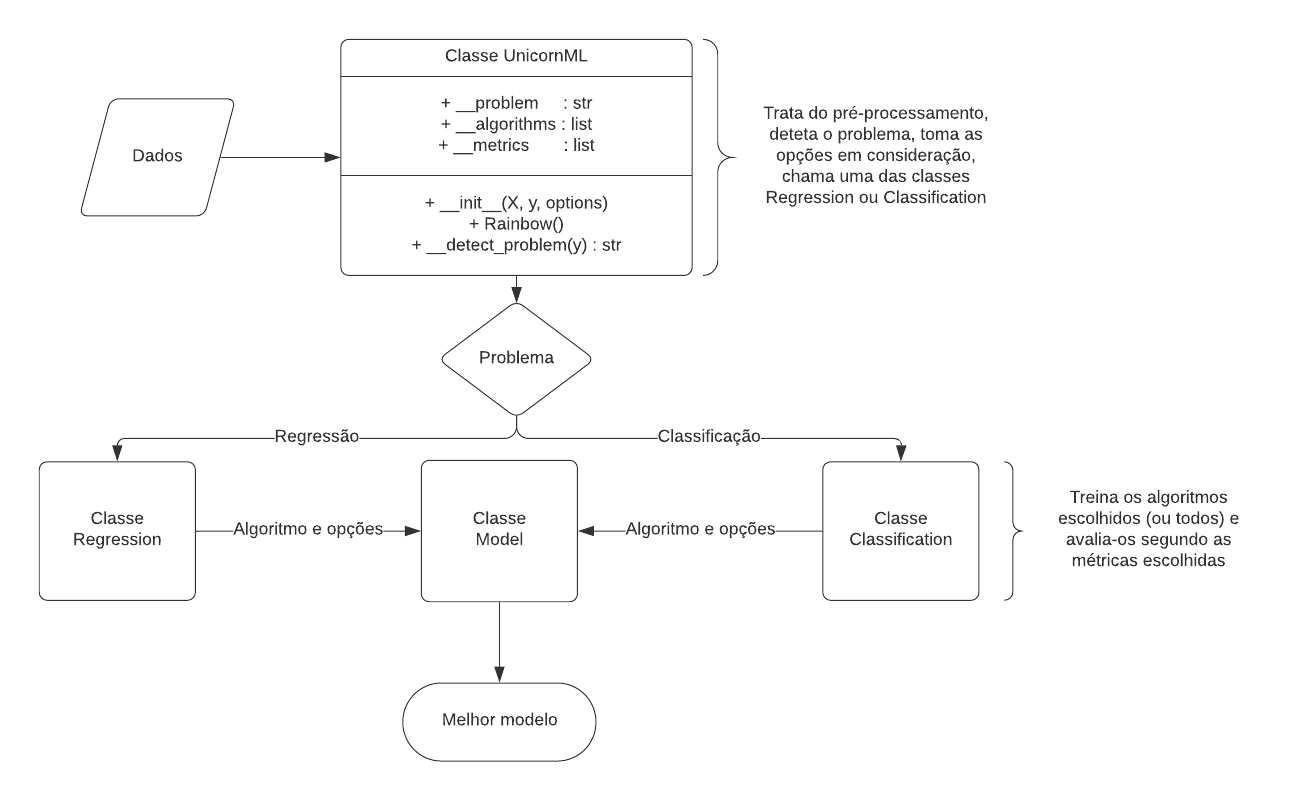
\includegraphics[width=1.0\textwidth]{Images/Diagram.png}
			\caption{Fluxo de execução da \textit{framework}}
			\label{fig:3}
		\end{figure}

		Posto isto, existe ainda um outro problema, tratado de forma diferente do que é exposto acima.
		Para o caso de imagens, o utilizador deve indicar, ao instanciar a classe principal, que o \textit{dataset} é de imagens, passando nas opções o formato das imagens - altura, largura e profundidade.
		A profundidade da imagem, entenda-se, corresponde ao facto de a imagem ter ou não cor, sendo igual a 3 no caso de ter (RGB).

		\subsection{Pré-processamento} \label{subsec:Pre-Processing}
		Na classe de pré-processamento realizam-se várias tarefas sobre os conjuntos de dados disponibilizados.
		Exibem-se de seguida as mesmas:

		\begin{itemize}
			\item Transformação dos dados:
			\begin{itemize}
				\item Separação entre os dados relativos às variáveis independentes dos dados associados à variável de interesse ou de saída;
				\item Tratamento de valores omissos: colunas com mais de 40\% de valores nulos são eliminadas. Os valores numéricos são substituídos pela média dos valores da coluna enquanto que os categóricos são alterados para a moda;
				\item Redimensionamento e normalização: utilização de mecanismos de \textit{scaling} e \textit{label encoding} da biblioteca \texttt{scikit-learn}.
			\end{itemize}
			\item Seleção de \textit{features}:
			\begin{itemize}
				\item Utilização do \textit{PCA} para obter os principais componentes das \textit{features} com maior correlação e, por isso, com maior relevância.
			\end{itemize}
			
		\end{itemize}

		\subsection{Problema} \label{subsec:Problem}
		Os problemas de aprendizagem supervisionada podem ser divididos em dois conjuntos: problemas de regressão e problemas de classificação.
		Como tal, é importante perceber-se qual dos dois problemas enfrentamos, de forma a que se possa poupar tempo e recursos de computação na procura do melhor modelo.
		Para isso, foi pensada uma forma de identificar o tipo do problema. No entanto, tal como referido na proposta já entregue, esta não é uma prioridade,
		pelo que o método para já utilizado é simples e identifica apenas a presença de inteiros ou \textit{floats} para fazer esta distinção.

		No entanto, este processamento é evitado se o utilizador indicar qual dos problemas os seus dados representam.
		Esta indicação é dada através de uma opção, sendo passada uma de duas \textit{strings}: \textit{\texttt{Regression}} ou \textit{\texttt{Classification}}.

		\subsection{Algoritmos} \label{subsec:Algorithms}
		A \textsl{UnicornML} oferece diversos algoritmos para cada um dos tipos de problemas. 
		O utilizador pode escolher, dentro dos algoritmos disponíveis, quais os que quer que sejam testados. 
		No entanto, os algoritmos só serão testados se estiverem disponíveis para o tipo de problema identificado pela \textit{framework} ou indicado pelo mesmo.

		Caso o utilizador não indique quais os algoritmos que prefere que sejam testados, a \textit{framework} testará todos os algoritmos disponíveis para o tipo de problema identificado pela mesma ou indicado pelo utilizador.
            
			\subsubsection{Classificação} \label{sssec:Classification1}
			Os algoritmos disponíveis para problemas de classificação são os seguintes:
			\begin{itemize}
				\item Regressão logística;
				\item \textit{K-Nearest Neighbors} (KNN);
				\item \textit{Support Vector Classifier} (SVC) - uma \textit{Support Vector Machine} (SVM) para classificação;
				\item \textit{kernel} SVM - uma SVM com uma função \textit{kernel}, que permite a classificação em espaços de dimensão superiores;
				\item Classificadores Bayesianos - família de classificadores baseados na teoria de Bayes. Foram implementados dois algoritmos distintos: \textit{Gaussian} e \textit{Bernoulli};
				\item Árvores de decisão;
				\item \textit{Random Forest} - operam construindo uma multitude de árvores de decisão.
				\item Redes neuronais artificiais.
			\end{itemize}

			Estes algoritmos encontram-se na classe \texttt{Classification}, tal como se pode observar na figura \hyperref[fig:1]{1}.

			\subsubsection{Regressão} \label{sssec:Regression1}
			Os algoritmos disponíveis para problemas de regressão são os seguintes:
			\begin{itemize}
				\item Regressão linear;
				\item \textit{Support Vector Regressor} (SVR) - uma SVM para regressão;
				\item Árvores de decisão;
				\item \textit{Random Forest} - operam construindo uma multitude de árvores de decisão;
				\item Redes neuronais artificiais.
			\end{itemize}

			Estes algoritmos encontram-se na classe \texttt{Regression}, presente na estrutura da \textit{framework} desta aplicação (consultar a figura \hyperref[fig:1]{1}).

		\subsection{Métricas} \label{subsec:Metrics}
		As métricas permitem avaliar o desempenho de um certo modelo. 
		O utilizador também pode escolher as métricas que irão ser tomadas em consideração e, posteriormente, apresentadas.
		Mais uma vez, isso está limitado às métricas disponíveis para cada tipo de problema.
		De realçar que nem todas as métricas podem estar disponíveis num determinado momento.

            \subsubsection{Classificação} \label{sssec:Classification2}
			As métricas disponíveis para problemas de classificação são as seguintes:
			\begin{itemize}
				\item \textit{Accuracy} - Percentagem de exemplos corretamente classificados (PECC). Esta métrica foi definida por defeito;
				\item \textit{Auc};
				\item \textit{Precision} - Valor preditivo positivo;
				\item \textit{Recall} - Sensibilidade.
			\end{itemize}

            \subsubsection{Regressão} \label{sssec:Regression2}
			As métricas disponíveis para problemas de regressão são as seguintes:
			\begin{itemize}
				\item \textit{Mean Square Error} (MSE) - métrica definida por defeito;
				\item \textit{Mean Absolute Error} (MAE);
				\item \textit{R-squared} ($R^{2}$).
			\end{itemize}

		\subsection{Modelo}
		A classe \texttt{Model}, em \texttt{unicornML/model/\_\_init\_\_.py}, é o coração de toda a \textit{framework}.
		A mesma foi pensada de forma a simplificar o restante código e reduzir duplicações do mesmo.
		Nesta são incorporados vários tipos de informação, nomeadamente o conjunto de dados (treino e teste), a métrica selecionada para realizar a estimação do erro associada ao modelo escolhido e, ainda, os resultados obtidos após efetuar a otimização dos hiperparâmetros.

			\subsubsection{Otimização de parâmetros} \label{sssec::optimization}
			A otimização de parâmetros procura o melhor modelo para cada um dos algoritmos.
			Sendo que após encontrar os melhores parâmetros para o estimador, é calculada a métrica desse estimador para os dados de teste.
			Esta métrica é adicionada a uma lista que contém todos os estimadores e os respetivos valores da métrica selecionada.

			Para as redes neuronais a otimização é realizada com a biblioteca \texttt{kerastuner}. Para os restantes algoritmos, a otimização é realizada pelo \texttt{RandomizedSearch}.


		\subsection{Imagens}
		A classe \texttt{Images}, em \texttt{unicornML/images/\_\_init\_\_.py}, é responsável pelo desenvolvimento de modelos para imagens.
		Esta classe é instanciada e usada exclusivamente pela classe principal e recebe a diretoria onde as mesmas estão presentes, o formato das imagens e, opcionalmente, se se quer realizar, ou não, \textit{fine tuning}.

		Importa realçar que a diretoria das imagens deve estar dividida em três pastas: \textit{test}, \textit{train} e \textit{validation}.

		Esta classe é capaz de, para o caso de existirem poucas imagens para treino, realizar o processo de \textit{Data Augmentation}, de forma a combater o sobre-ajustamento e melhorar a qualidade do modelo.

		Pela complexidade e poder computacional que a classificação de imagens exige, foi decidido o uso de uma rede pré-treinada, tendo-se escolhido a rede \texttt{VGG16}, não incluindo o topo da mesma.
		Por este motivo, aparece a última opção, que indica se se quer re-treinar as últimas camadas da rede pré-treinada.

		No topo da rede \texttt{VGG16}, são adicionadas um camada \texttt{Flatten} e duas camadas \texttt{Dense}: a primeira com 256 neurónios e função de ativação \texttt{relu} e a segunda com apenas 1 neurónio e função de ativação \texttt{sigmoid}.
		A última camada representa a camada de saída.

		Por fim é possível treinar e avaliar a performance do modelo.
}

\chapter{Testes e análise de resultados} \label{ch:Test&Analysis}
\large{
	Para validar todos os aspetos considerados durante a implementação deste trabalho, foram incorporados nesta \textit{framework} vários conjuntos de dados que servem de teste à mesma.
	Como tal, foram adicionados no total 12 conjuntos de dados distintos entre si, havendo tanto problemas de regressão como de classificação com múltiplas classes a serem modelados.
	Estes conjuntos de dados foram obtidos em https://machinelearningmastery.com/standard-machine-learning-datasets, sendo que alguns deles contêm informação sobre os valores esperados da precisão do modelo gerado. Assim, faremos uma comparação dos resultados obtidos com os esperados para alguns destes dados.

	De forma a exibir apenas alguns dos resultados obtidos, expõem-se agora os conjuntos de dados considerados para o efeito. Para cada um, é indicado o valor mínimo esperado (e os melhores resultados, no caso de existirem). São ainda apresentados os valores obtidos pela nossa framework, tanto na fase da optimização dos hiperparâmetros como o treino com todos os dados disponíveis:
	\begin{itemize}
		\item \textsl{Pima Indians Diabetes Dataset}
		Desempenho mínimo esperado: 65\%. Melhores resultados previstos: 77\%.
		Resultado: 80.5\% (accuracy 76.5\%), Gaussian Nayve Bayes
		\item \textsl{Sonar Dataset}
		Desempenho mínimo esperado: 53\%. Melhores resultados previstos: 88\%.
		Resultado: 83\% (accuracy 96.6\%), KNN
		\item \textsl{Banknote Dataset}
		Desempenho mínimo esperado: 50\%.
		Resultado: 97.8\% (accuracy 98\%), Logistic Regression 
		\item \textsl{Iris Flowers Dataset}
		Desempenho mínimo esperado: 26\%.
		Resultado: 93.3\% (accuracy 98.7\%), Decision Tree Classification
		\item \textsl{Abalone Dataset}
		Desempenho mínimo esperado: 16\%.
		Resultado: 27.5\% (accuracy 28.4\%), Kernel Support Vector Machine
		\item \textsl{Ionosphere Dataset}
		Desempenho mínimo esperado: 64\%. Melhores resultados previstos: 94\%.
		Resultado: 93.3\% (accuracy 98.7\%), Decision Tree Classifier
		\item \textsl{Wheat Seeds Dataset}
		Desempenho mínimo esperado: 28\%.
		Resultado: 95.2\% (accuracy 91.4\%), Neural Network
		\item \textsl{Imagens Gatos e Cães}
		Desempenho mínimo esperado: 95\%.
		Resultado: 87.5\%, CNN
	\end{itemize}

	Como pode ser notado, quase todos os casos obtiveram valores muito superiores ao esperado, o que demonstra as vantagens da nossa framework quando comparada com a otimização manual de hiperparâmetros.
	A única exceção foi o conjunto de imagens dos gatos e cães, onde o resultado obtivo foi um pouco inferior ao esperado. Isto deve-se a ter sido utilizado um subconjunto parcial dos dados totais e a rede ter sido treinada durante apenas uma época. Imposemos esta restrição para este caso específico para acelerar o processo de treino, mas note-se que não é um problema da framework em si.
}

\chapter{Conclusão} \label{ch:Conclusion}
\large{
	Finalizado o trabalho, temos a referir que, apesar de no início termos ficado um pouco apreensivos quanto ao tema escolhido para o trabalho, estamos muito satisfeitos com o trabalho desenvolvido. 
	Assim, reforçamos a nossa escolha da opção de trabalho prático.

	Este trabalho deu-nos a oportunidade de abordar quase toda a matéria lecionada nas aulas, enquanto que, se tivéssemos escolhido a outra opção, não teríamos tanta abrangência.
	A escolha do desenvolvimento de uma \textit{framework} de AutoML, a nosso ver, permite o tratamento de um grande conjunto de problemas sem grande interação do utilizador, o que leva a que indivíduos sem conhecimentos de \textit{machine learning} possam ter acesso à área.
	
	Analisando os objetivos inicialmente traçados e aprensentados na proposta inicial, podemos afirmar que estes foram cumpridos e até superados.
	O pré-processamento dos dados era, inicialmente, um projeto futuro. 
	No entanto, está totalmente implementado, o que permite maior flexibilidade e, principalmente, o combate ao \textit{overfitting}.
	O desenvolvimento de modelos de classificação de imagens era algo que não estava inicialmente previsto e que foi implementado, adicionando também aos objetivos iniciais.

	Quanto aos resultados obtidos, temos a referir que foram muito positivos, visto que ultrapassámos muitos dos valores obtidos de forma manual. Isto é mais uma prova do excelente funcionamento da \textit{framework}.
	
	Para concluir, há apenas que referir que o trabalho como um todo superou as nossas expetativas, tendo em conta a modularidade/simplicidade do código e os resultados obtidos.
}

\appendix
\chapter{Documentação} \label{ch:Documentation}
\begin{itemize}
    \item \textit{Python} 3:
	\par \textit{\url{https://docs.python.org/3/}}
	\item \textit{Pandas}:
	\par \textit{\url{https://pandas.pydata.org/docs/}}
	\item \textit{Numpy}:
	\par \textit{\url{https://numpy.org/doc/}}
	\item \textit{Scipy}:
	\par \textit{\url{https://docs.scipy.org/doc/scipy/reference/}}
	\item \textit{Scikit-learn} - \textit{supervised learning}:
	\sloppy
	\par \textit{\url{https://scikit-learn.org/stable/supervised_learning.html\#supervised-learning}}
	\item \textit{Scikit-learn} (\textsl{API}):
    \par \textit{\url{https://scikit-learn.org/stable/modules/classes.html}}
	\item \textit{Tensorflow} - \texttt{keras}:
	\par \textit{\url{https://www.tensorflow.org/api_docs/python/tf/keras}}
	\item \textit{Kerastuner}:
	\par \textit{\url{https://keras-team.github.io/keras-tuner/}}
\end{itemize}

\end{document}